\section{Proposed Research}
\label{sec:proposedresearch}

To motivate the need for better data race detection techniques for structured
parallelism (i.e. OpenMP), rather than classic techniques such as
happens-before relation, consider the example in Figure~\ref{fig:nested}.
%


\begin{figure}
  \centering
  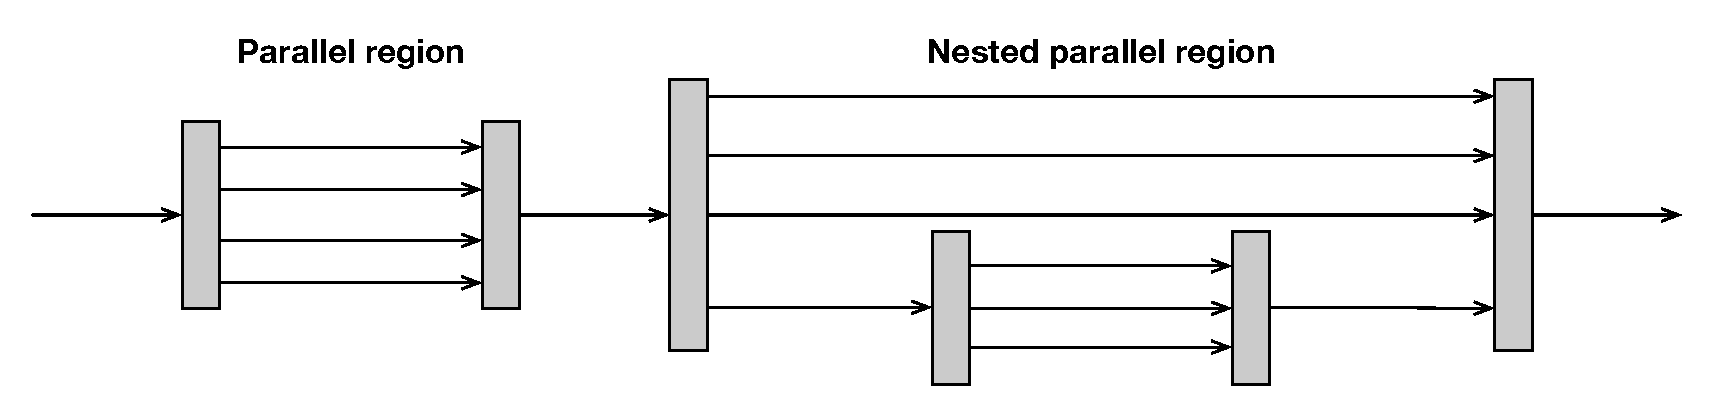
\includegraphics[width=0.95\textwidth]{figures/nested_parallelism}
  \caption{OpenMP nested parallelism}
  \label{fig:nested}
\end{figure}

\begin{itemize}
\item Static + dynamic analysis
\item Sequential blacklisting due to OpenMP structured parallelism
\item Barrier intervals
\item labeling to identify concurrent threads
\item sort of lock-set
\item Implemented by central but fast data structure
\item OMPT/OMPD
\end{itemize}

%%% Local Variables:
%%% mode: latex
%%% eval: (flyspell-mode 1)
%%% TeX-master: "root.tex"
%%% End:
